\documentclass[12pt,pdf,hyperref={unicode}]{beamer}


%\documentclass[10pt]{beamer}

\usetheme[progressbar=frametitle]{metropolis}

\usepackage{booktabs}
\usepackage[scale=2]{ccicons}

\usepackage{pgfplots}
\usepgfplotslibrary{dateplot}

\usepackage{xspace}
\newcommand{\themename}{\textbf{\textsc{metropolis}}\xspace}


%\usepackage{lmodern}

% подключаем кириллицу 
\usepackage[T2A]{fontenc}
\usepackage[utf8]{inputenc}
\usepackage{listings}
%\usepackage{graphicx}
\usepackage{hyperref}

% отключить клавиши навигации
\setbeamertemplate{navigation symbols}{}

% тема оформления
\usetheme{Pittsburgh}

% цветовая схема
\usecolortheme{default}

\definecolor{light-gray}{gray}{0.90}

\title{Семинар №8}   
\subtitle{ФАКИ \the\year}
\author{Бирюков В. А.} 
\date{\today}
% \logo{
\includegraphics[height=5mm]{images/logo.png}\vspace{-7pt}}

\begin{document}

\lstset{language=C}

% титульный слайд
\begin{frame}
\titlepage
\end{frame} 

\defverbatim[colored]\makeset{
\begin{lstlisting}[language=C++,basicstyle=\ttfamily,keywordstyle=\color{blue}]
void make_set(int X) {
  parent[X] = X;
}
\end{lstlisting}
}

\lstset{
  language=C,                % choose the language of the code
  keywordstyle=\color{blue},
  numbers=none,                   % where to put the line-numbers
  stepnumber=1,                   % the step between two line-numbers.        
  numbersep=5pt,                  % how far the line-numbers are from the code
  backgroundcolor=\color{light-gray},  % choose the background color. You must add \usepackage{color}
  showspaces=false,               % show spaces adding particular underscores
  showstringspaces=false,         % underline spaces within strings
  showtabs=false,                 % show tabs within strings adding particular underscores
  tabsize=2,                      % sets default tabsize to 2 spaces
  captionpos=b,                   % sets the caption-position to bottom
  breaklines=true,                % sets automatic line breaking
  breakatwhitespace=true,         % sets if automatic breaks should only happen at whitespace
}


\section{Указатели и память}

\begin{frame}[fragile]
\frametitle{Типы указателей} 
\begin{center}

\includegraphics[width=0.95\linewidth]{images/pointer_types.png}
\end{center}
\end{frame}



\begin{frame}[fragile]
\frametitle{Приведение указателей} 
\begin{itemize}
\item Приведение типов int и float: \\
\begin{lstlisting}[language=C++,basicstyle=\ttfamily,keywordstyle=\color{blue}]
float x = 5.2;
int y = (int)x;       // explicit
int z = x;            // implicit
\end{lstlisting}
\item Верно и для указателей: \\
\begin{lstlisting}[language=C++,basicstyle=\ttfamily,keywordstyle=\color{blue}]
float a;
float* pf = &a;
int* p1 = (int*)pf;   // explicit
int* p2 = pf;         // implicit
\end{lstlisting}
\end{itemize}
\end{frame}


\begin{frame}[fragile]
\frametitle{Указатели и память} 
\begin{center}
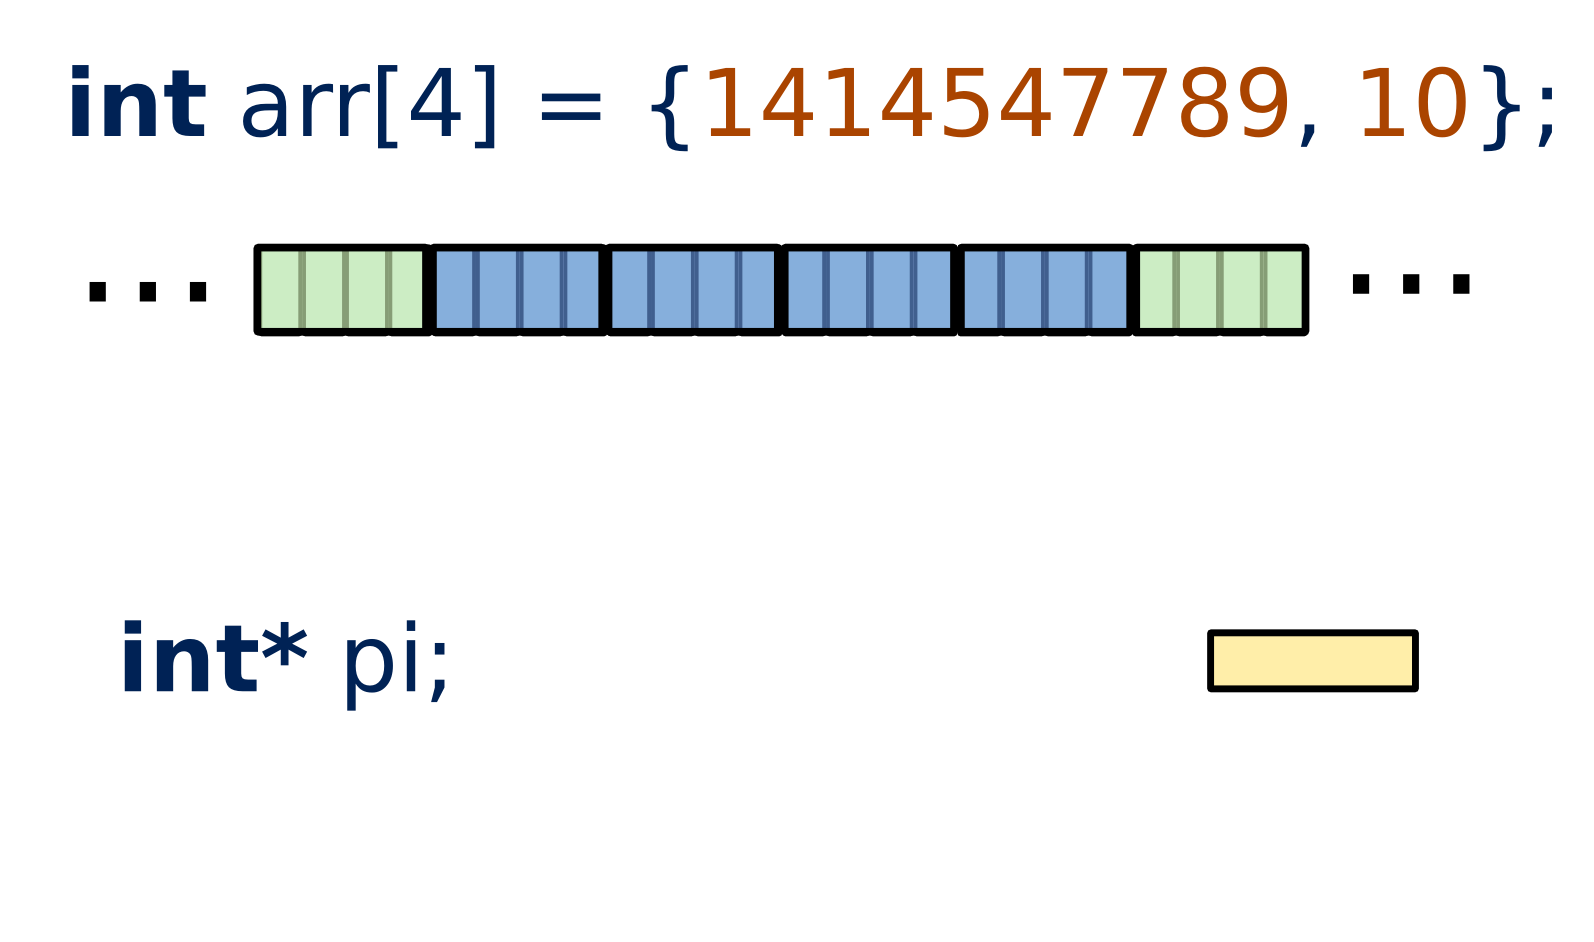
\includegraphics[width=0.95\linewidth]{images/memory_different_pointers_1.png}
\end{center}
\end{frame}

\begin{frame}[fragile]
\frametitle{Указатели и память} 
\begin{center}
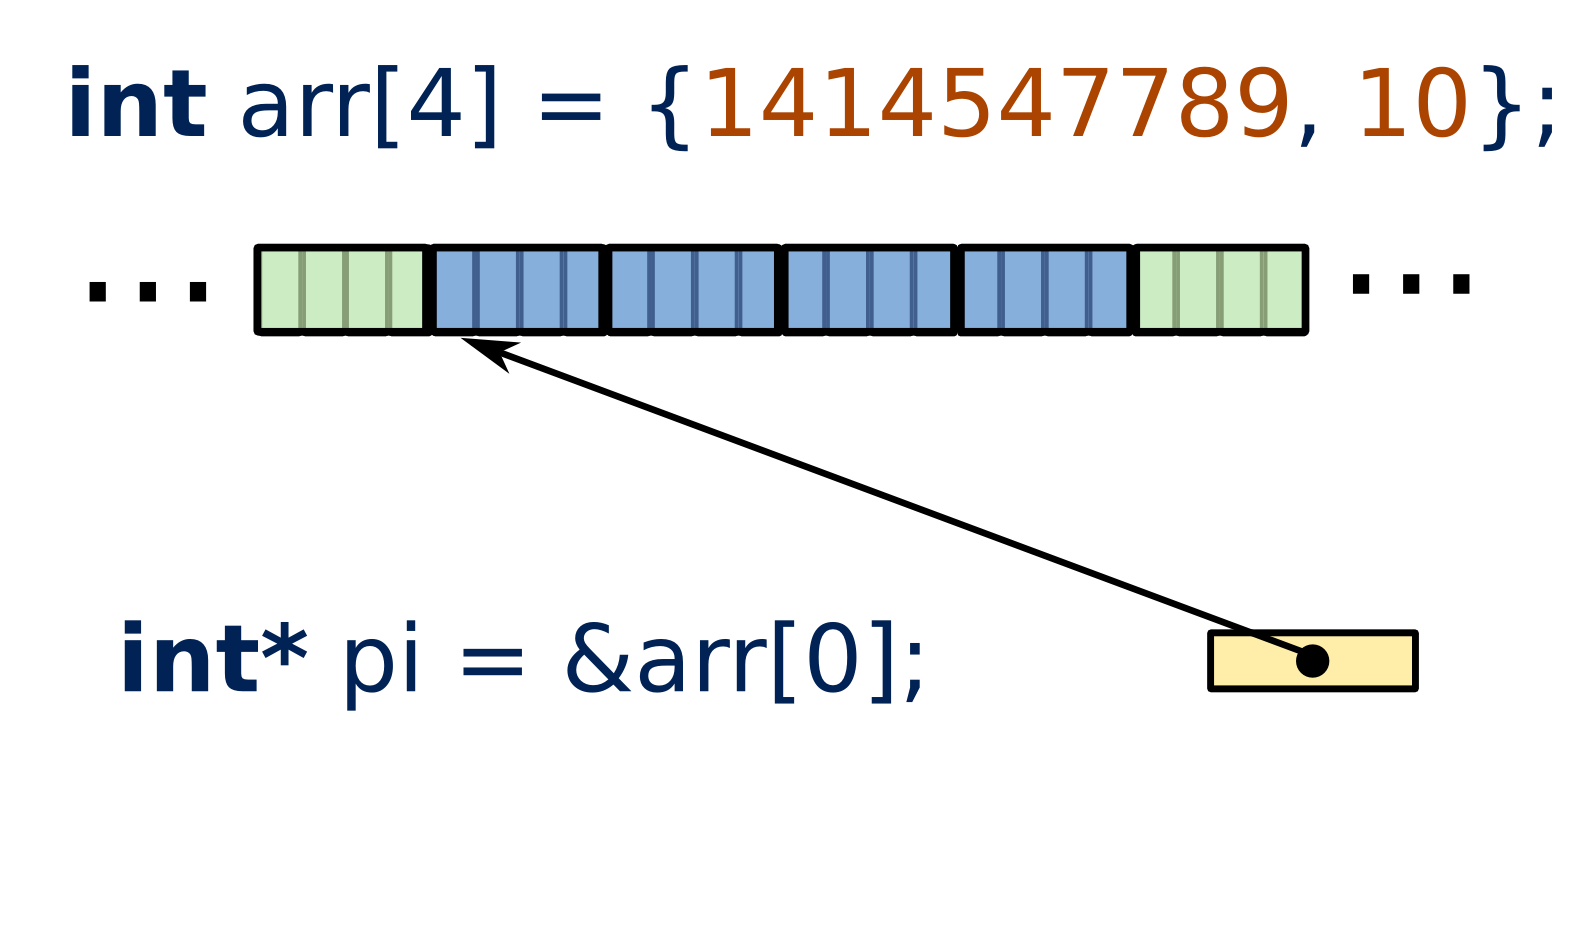
\includegraphics[width=0.95\linewidth]{images/memory_different_pointers_2.png}
\end{center}
\end{frame}

\begin{frame}[fragile]
\frametitle{Указатели и память. Арифметика указателей.} 
\begin{center}
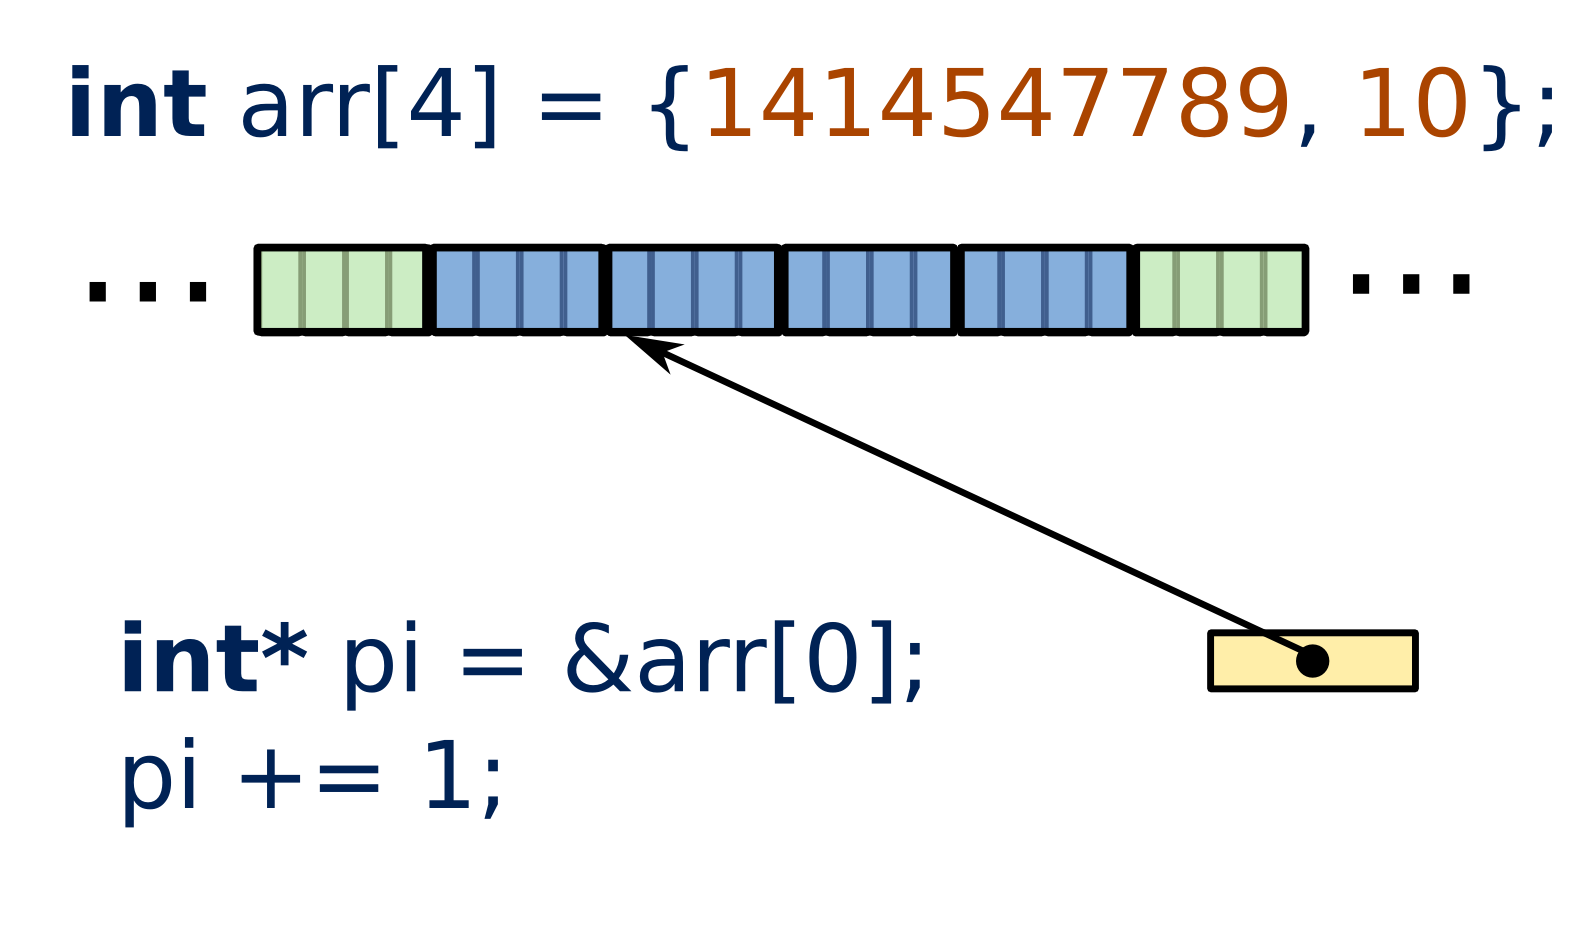
\includegraphics[width=0.95\linewidth]{images/memory_different_pointers_3a.png}
\end{center}
\end{frame}

\begin{frame}[fragile]
\frametitle{Указатели и память. Арифметика указателей.} 
\begin{center}
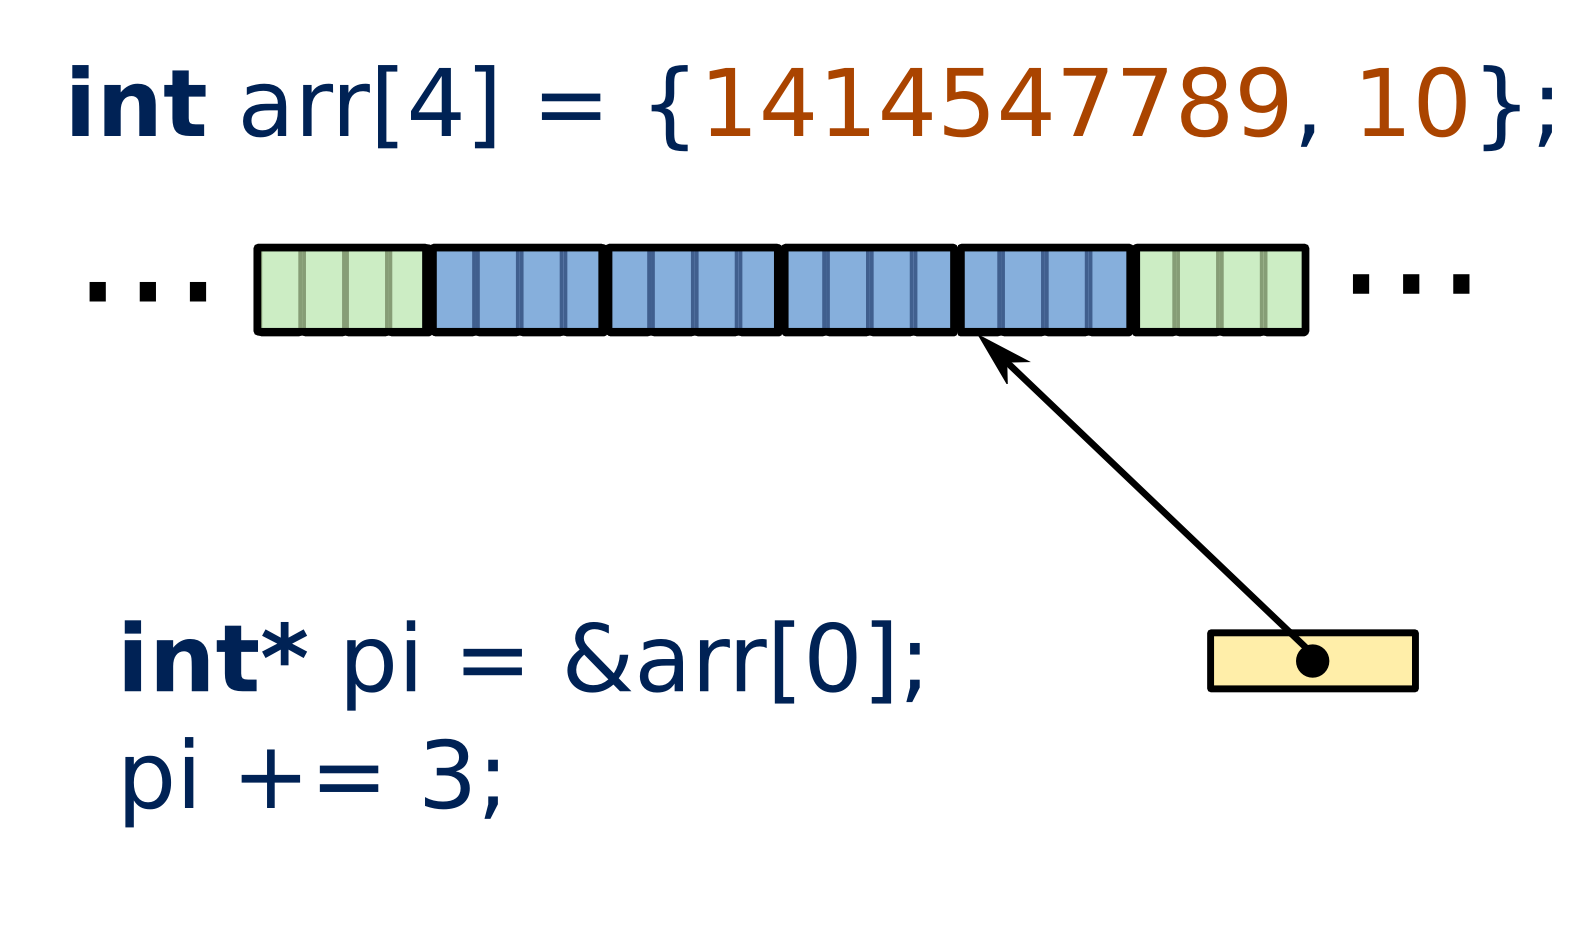
\includegraphics[width=0.95\linewidth]{images/memory_different_pointers_3b.png}
\end{center}
\end{frame}

\begin{frame}[fragile]
\frametitle{Указатели и память. Арифметика указателей.} 
\begin{center}
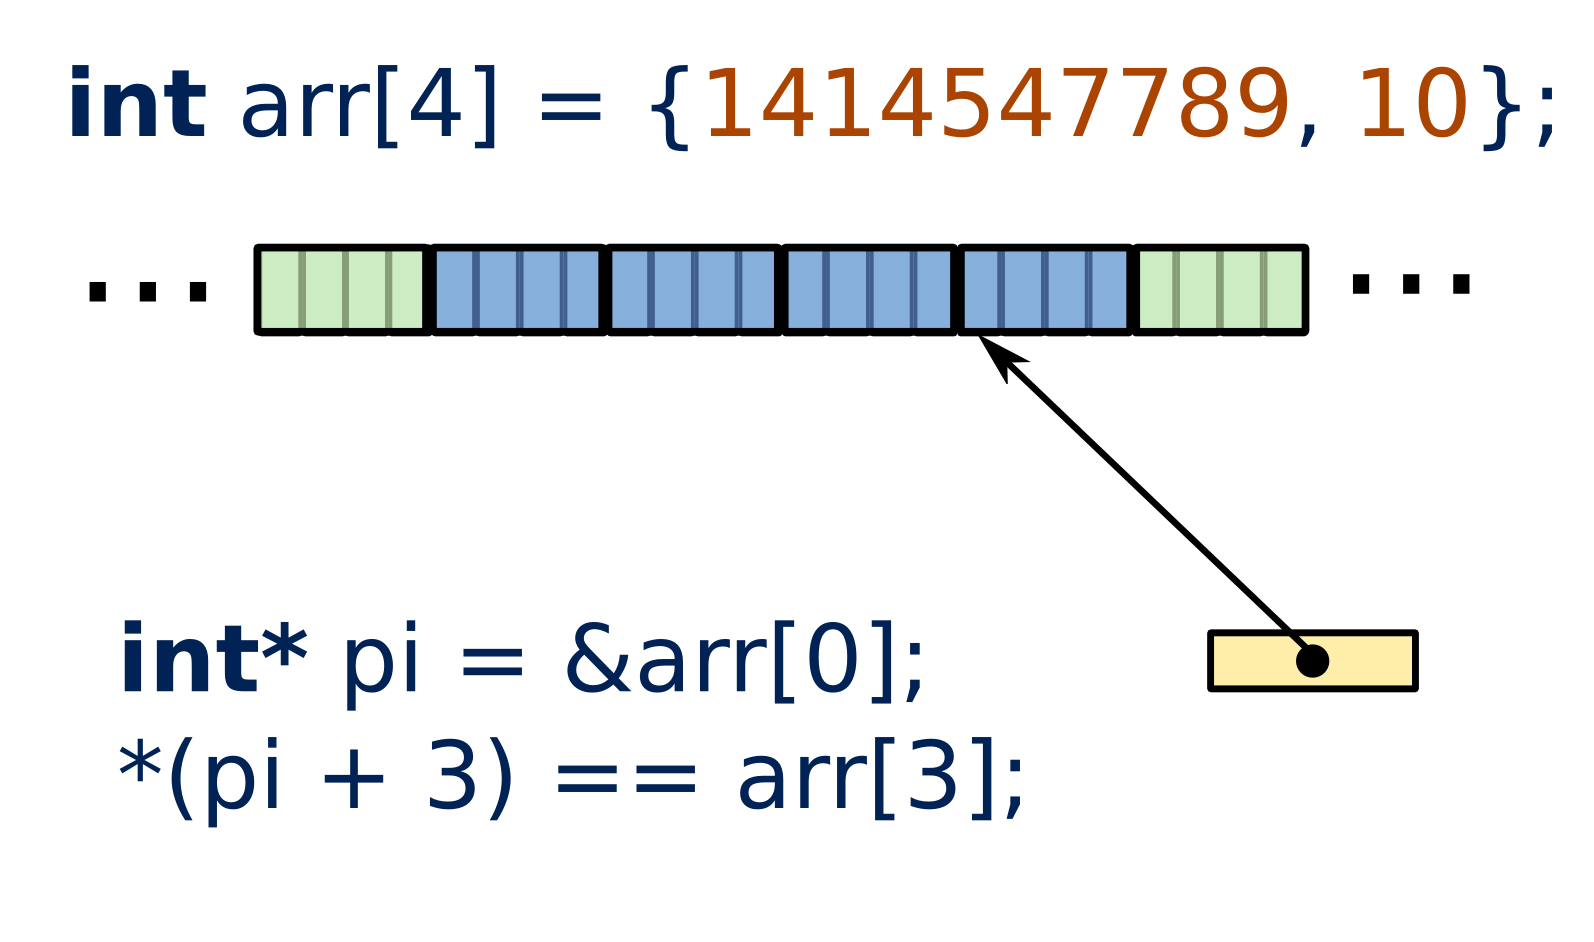
\includegraphics[width=0.95\linewidth]{images/memory_different_pointers_3c.png}
\end{center}
\end{frame}


\begin{frame}[fragile]
\frametitle{Указатели и память} 
\begin{center}

\includegraphics[width=0.95\linewidth]{images/arr_pointer_equality.png}
\end{center}
\end{frame}


\section{Указатель char* на int}

\begin{frame}[fragile]
\frametitle{Указатели и память} 
\begin{center}
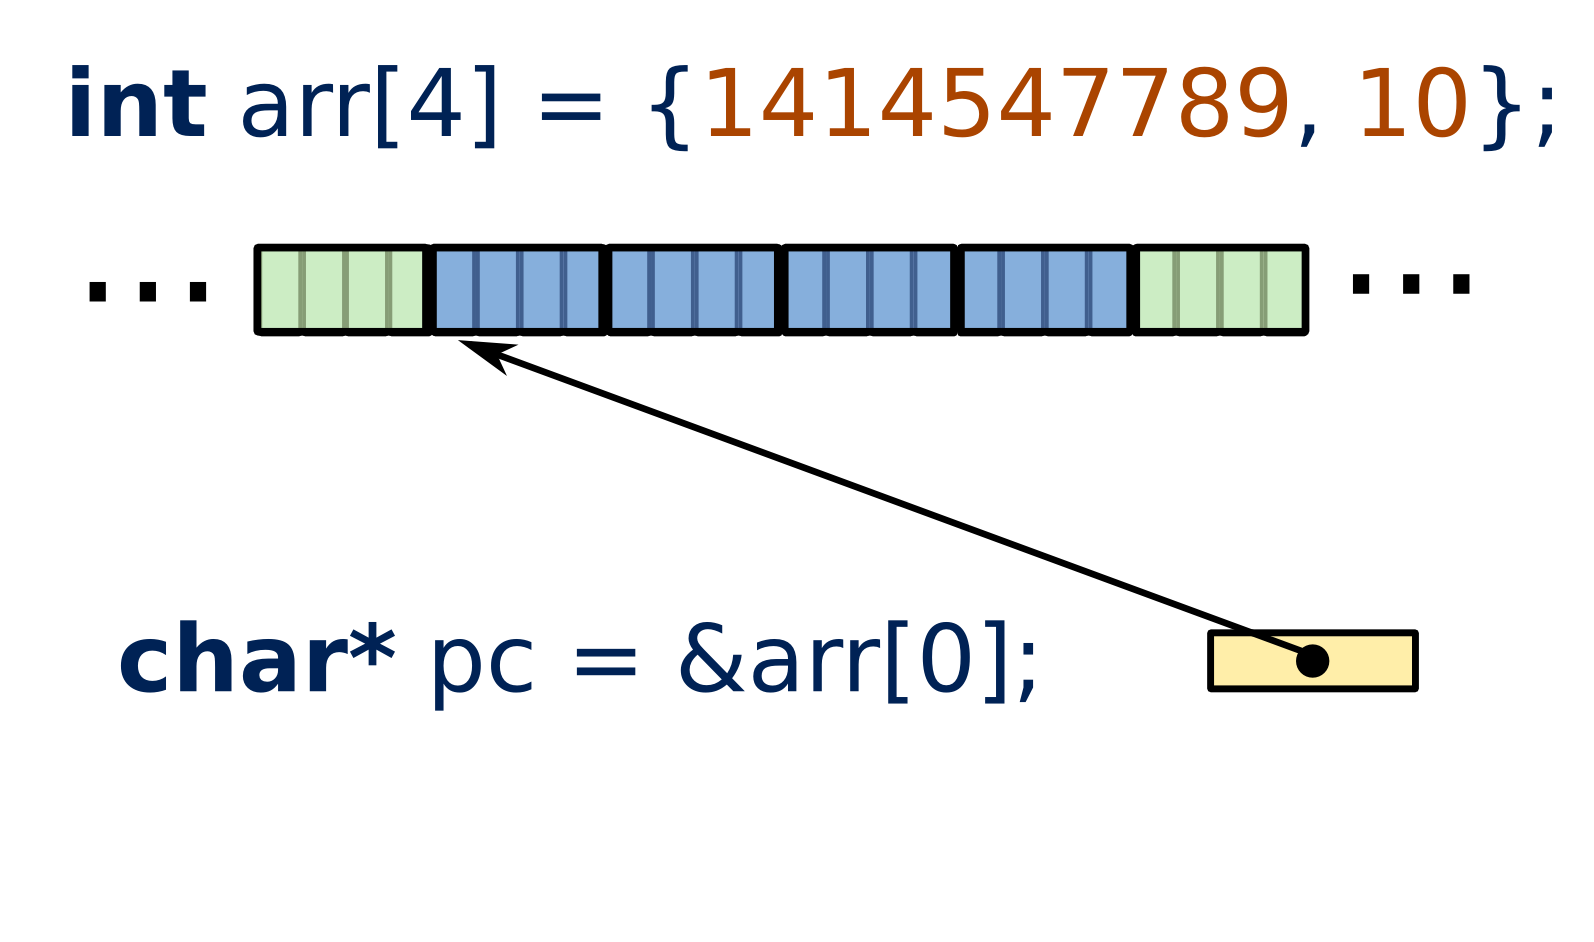
\includegraphics[width=0.95\linewidth]{images/memory_different_pointers_4a.png}
\end{center}
Примечание: при решении реальных задач присваивать указатели разных типов нежелательно.
\end{frame}

\begin{frame}[fragile]
\frametitle{Указатели и память} 
\begin{center}
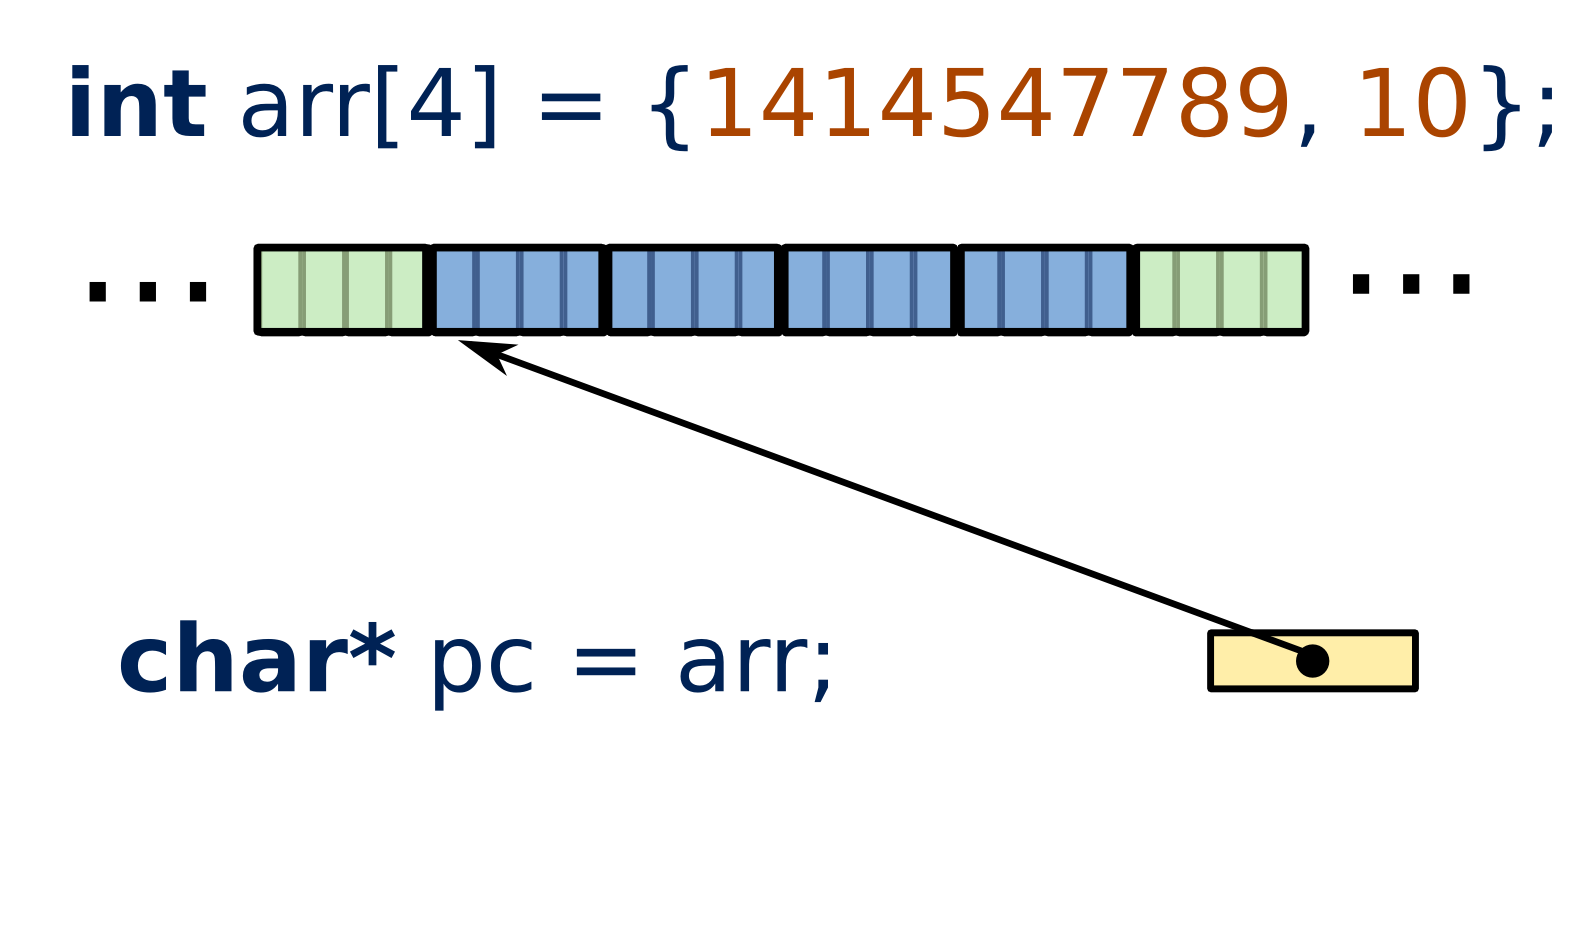
\includegraphics[width=0.95\linewidth]{images/memory_different_pointers_4b.png}
\end{center}
\end{frame}

\begin{frame}[fragile]
\frametitle{Указатели и память} 
\begin{center}
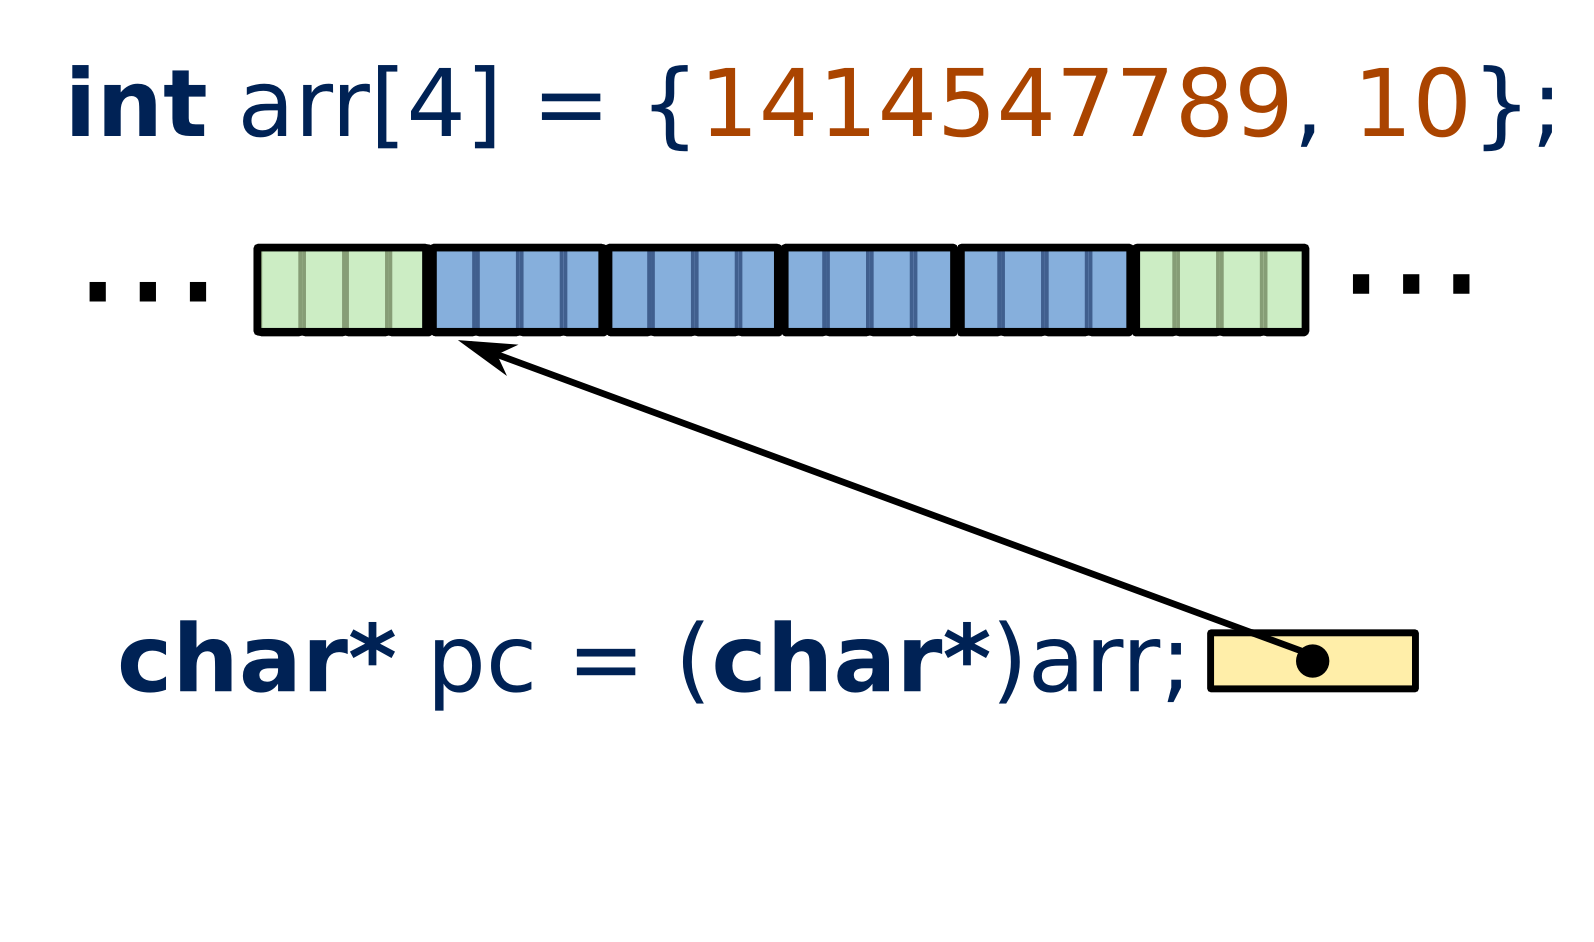
\includegraphics[width=0.95\linewidth]{images/memory_different_pointers_4c.png}
\end{center}
\end{frame}

\begin{frame}[fragile]
\frametitle{Указатели и память} 
\begin{center}
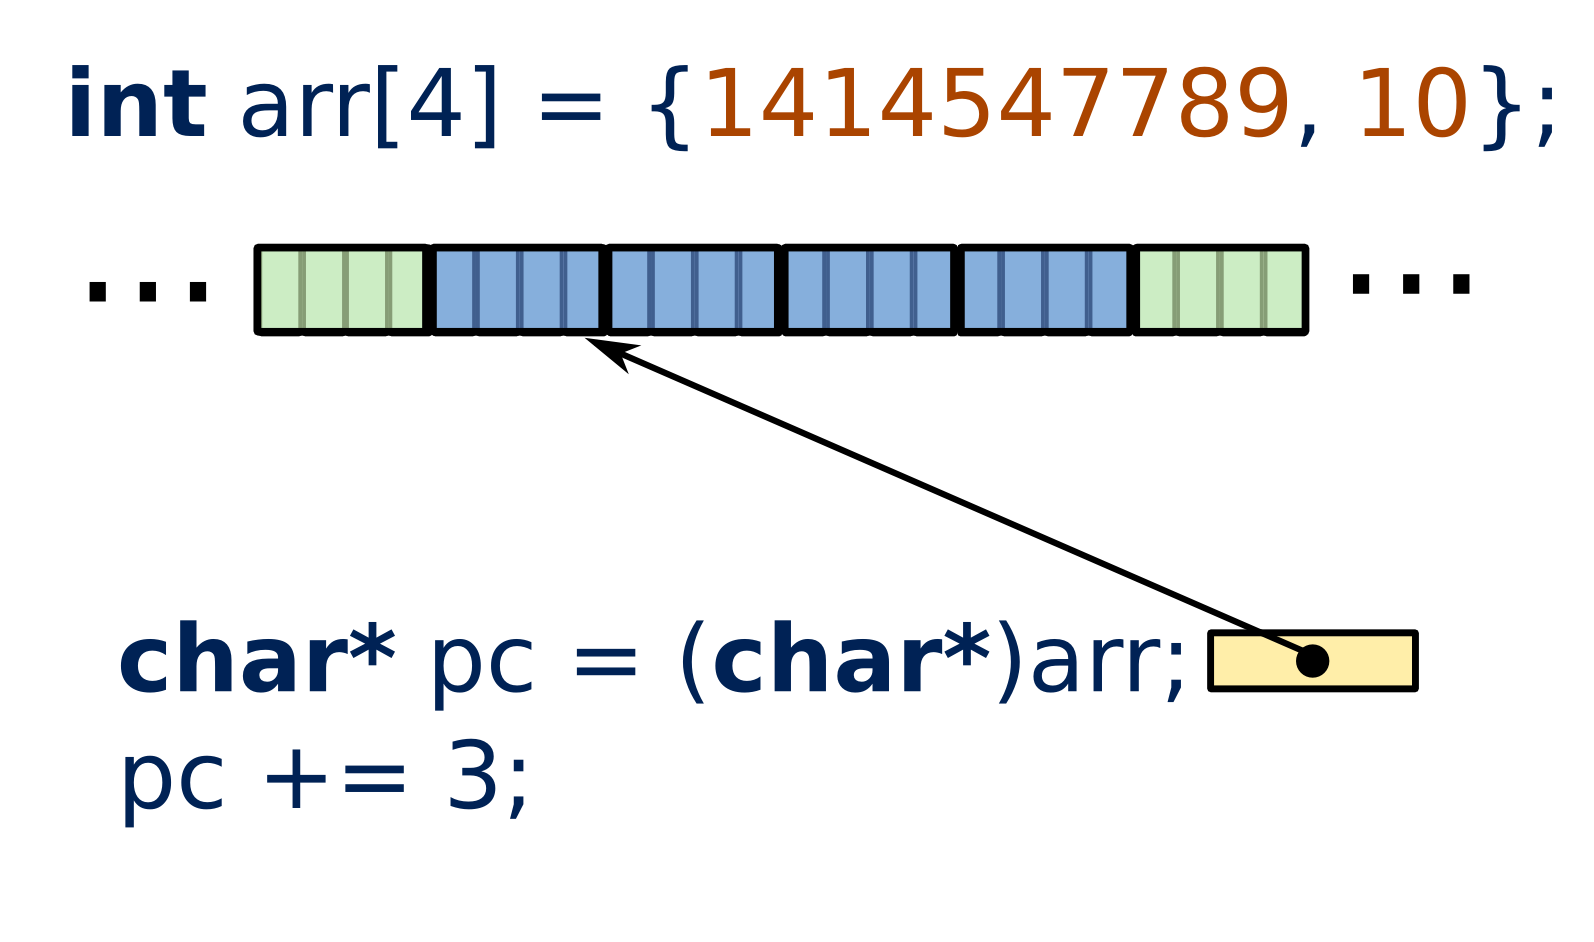
\includegraphics[width=0.95\linewidth]{images/memory_different_pointers_4e.png}
\end{center}
\end{frame}

\begin{frame}[fragile]
\frametitle{Указатели и память} 
\begin{center}
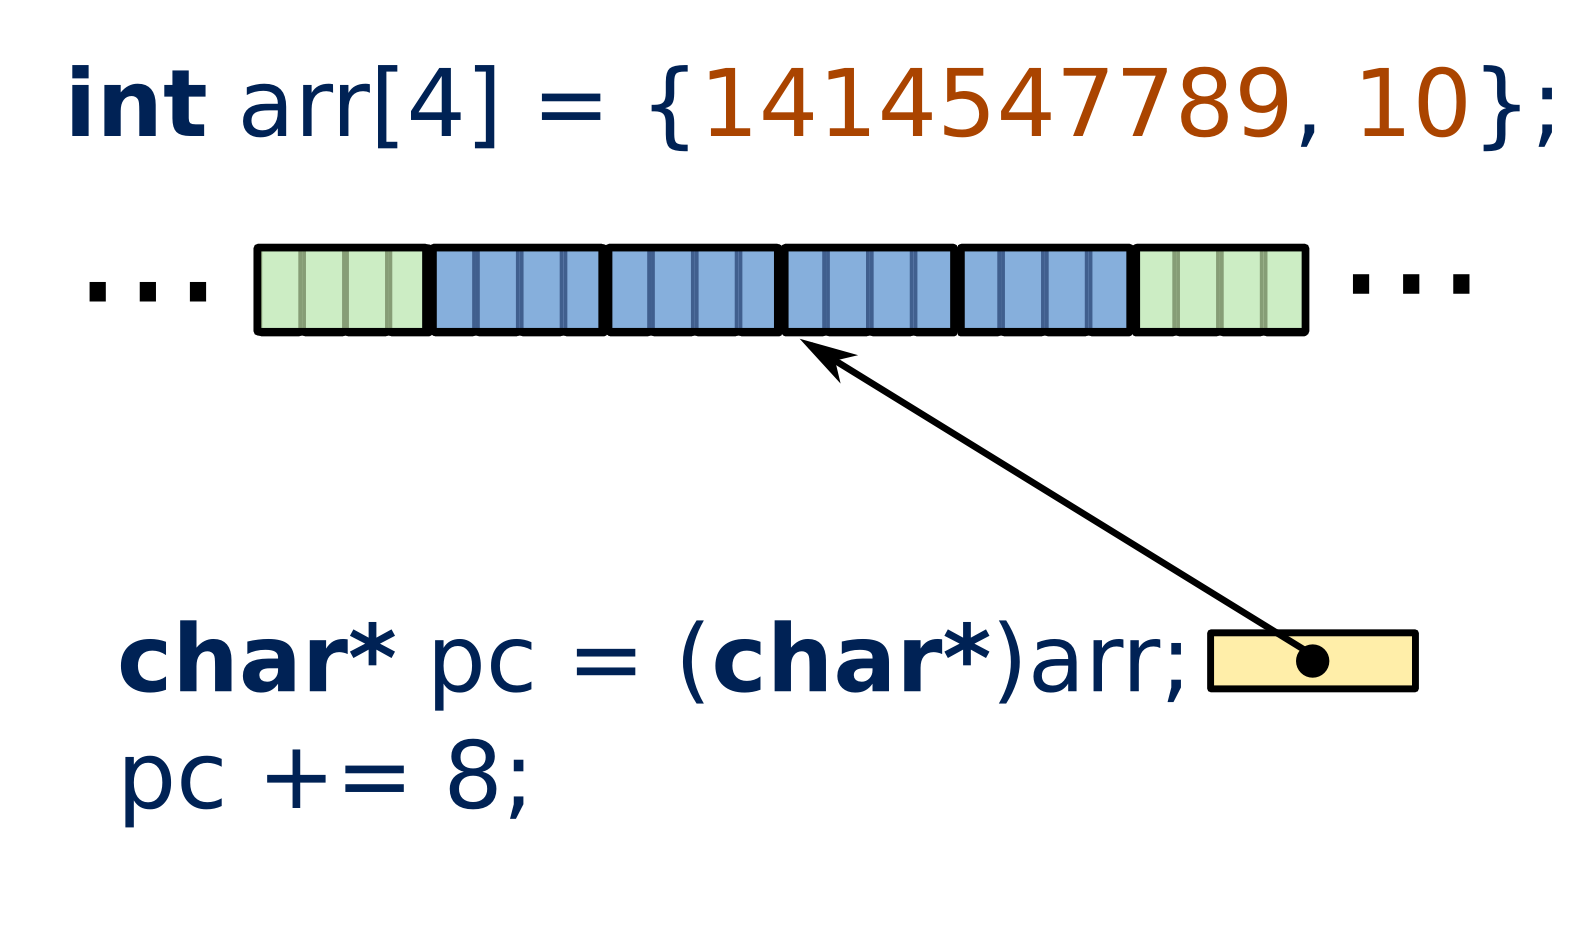
\includegraphics[width=0.95\linewidth]{images/memory_different_pointers_4f.png}
\end{center}
\end{frame}

\begin{frame}[fragile]
\frametitle{Указатели и память} 
\begin{center}
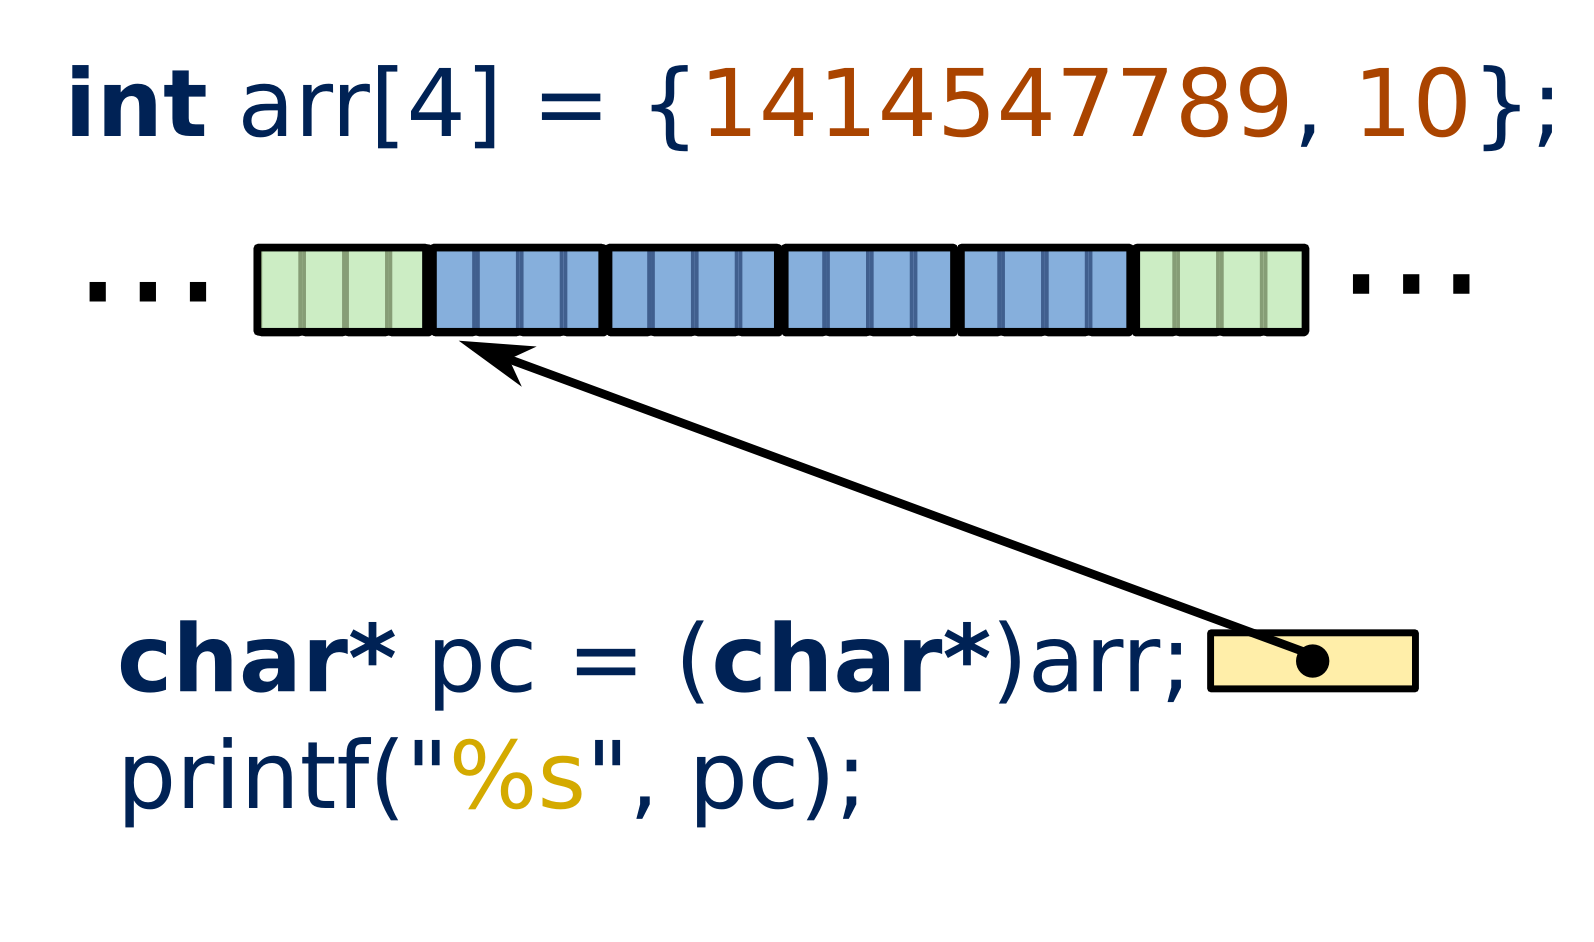
\includegraphics[width=0.95\linewidth]{images/memory_different_pointers_4g.png}
\end{center}
\end{frame}







\section{Malloc = Memory allocation}

\begin{frame}[fragile]
\frametitle{Функции для динамического выделения памяти} 
Нужно подключить библиотеку stdlib.h
\begin{itemize}
\item \textbf{void*} malloc(\textbf{size\_t} n) -- выделяет n байт и возвращает указатель \textbf{void*}
на начало этой памяти \\
\item \textbf{void} free(\textbf{void*} p) -- освобождает выделенную память\\
\item \textbf{void*} realloc (\textbf{void*} p, \textbf{size\_t} new\_n) -- перевыделяет выделенную память\\
\end{itemize}
Если забудите освободить выделенную память произойдёт утечка памяти.
\end{frame}

\begin{frame}[fragile]
\frametitle{Malloc} 
\begin{center}
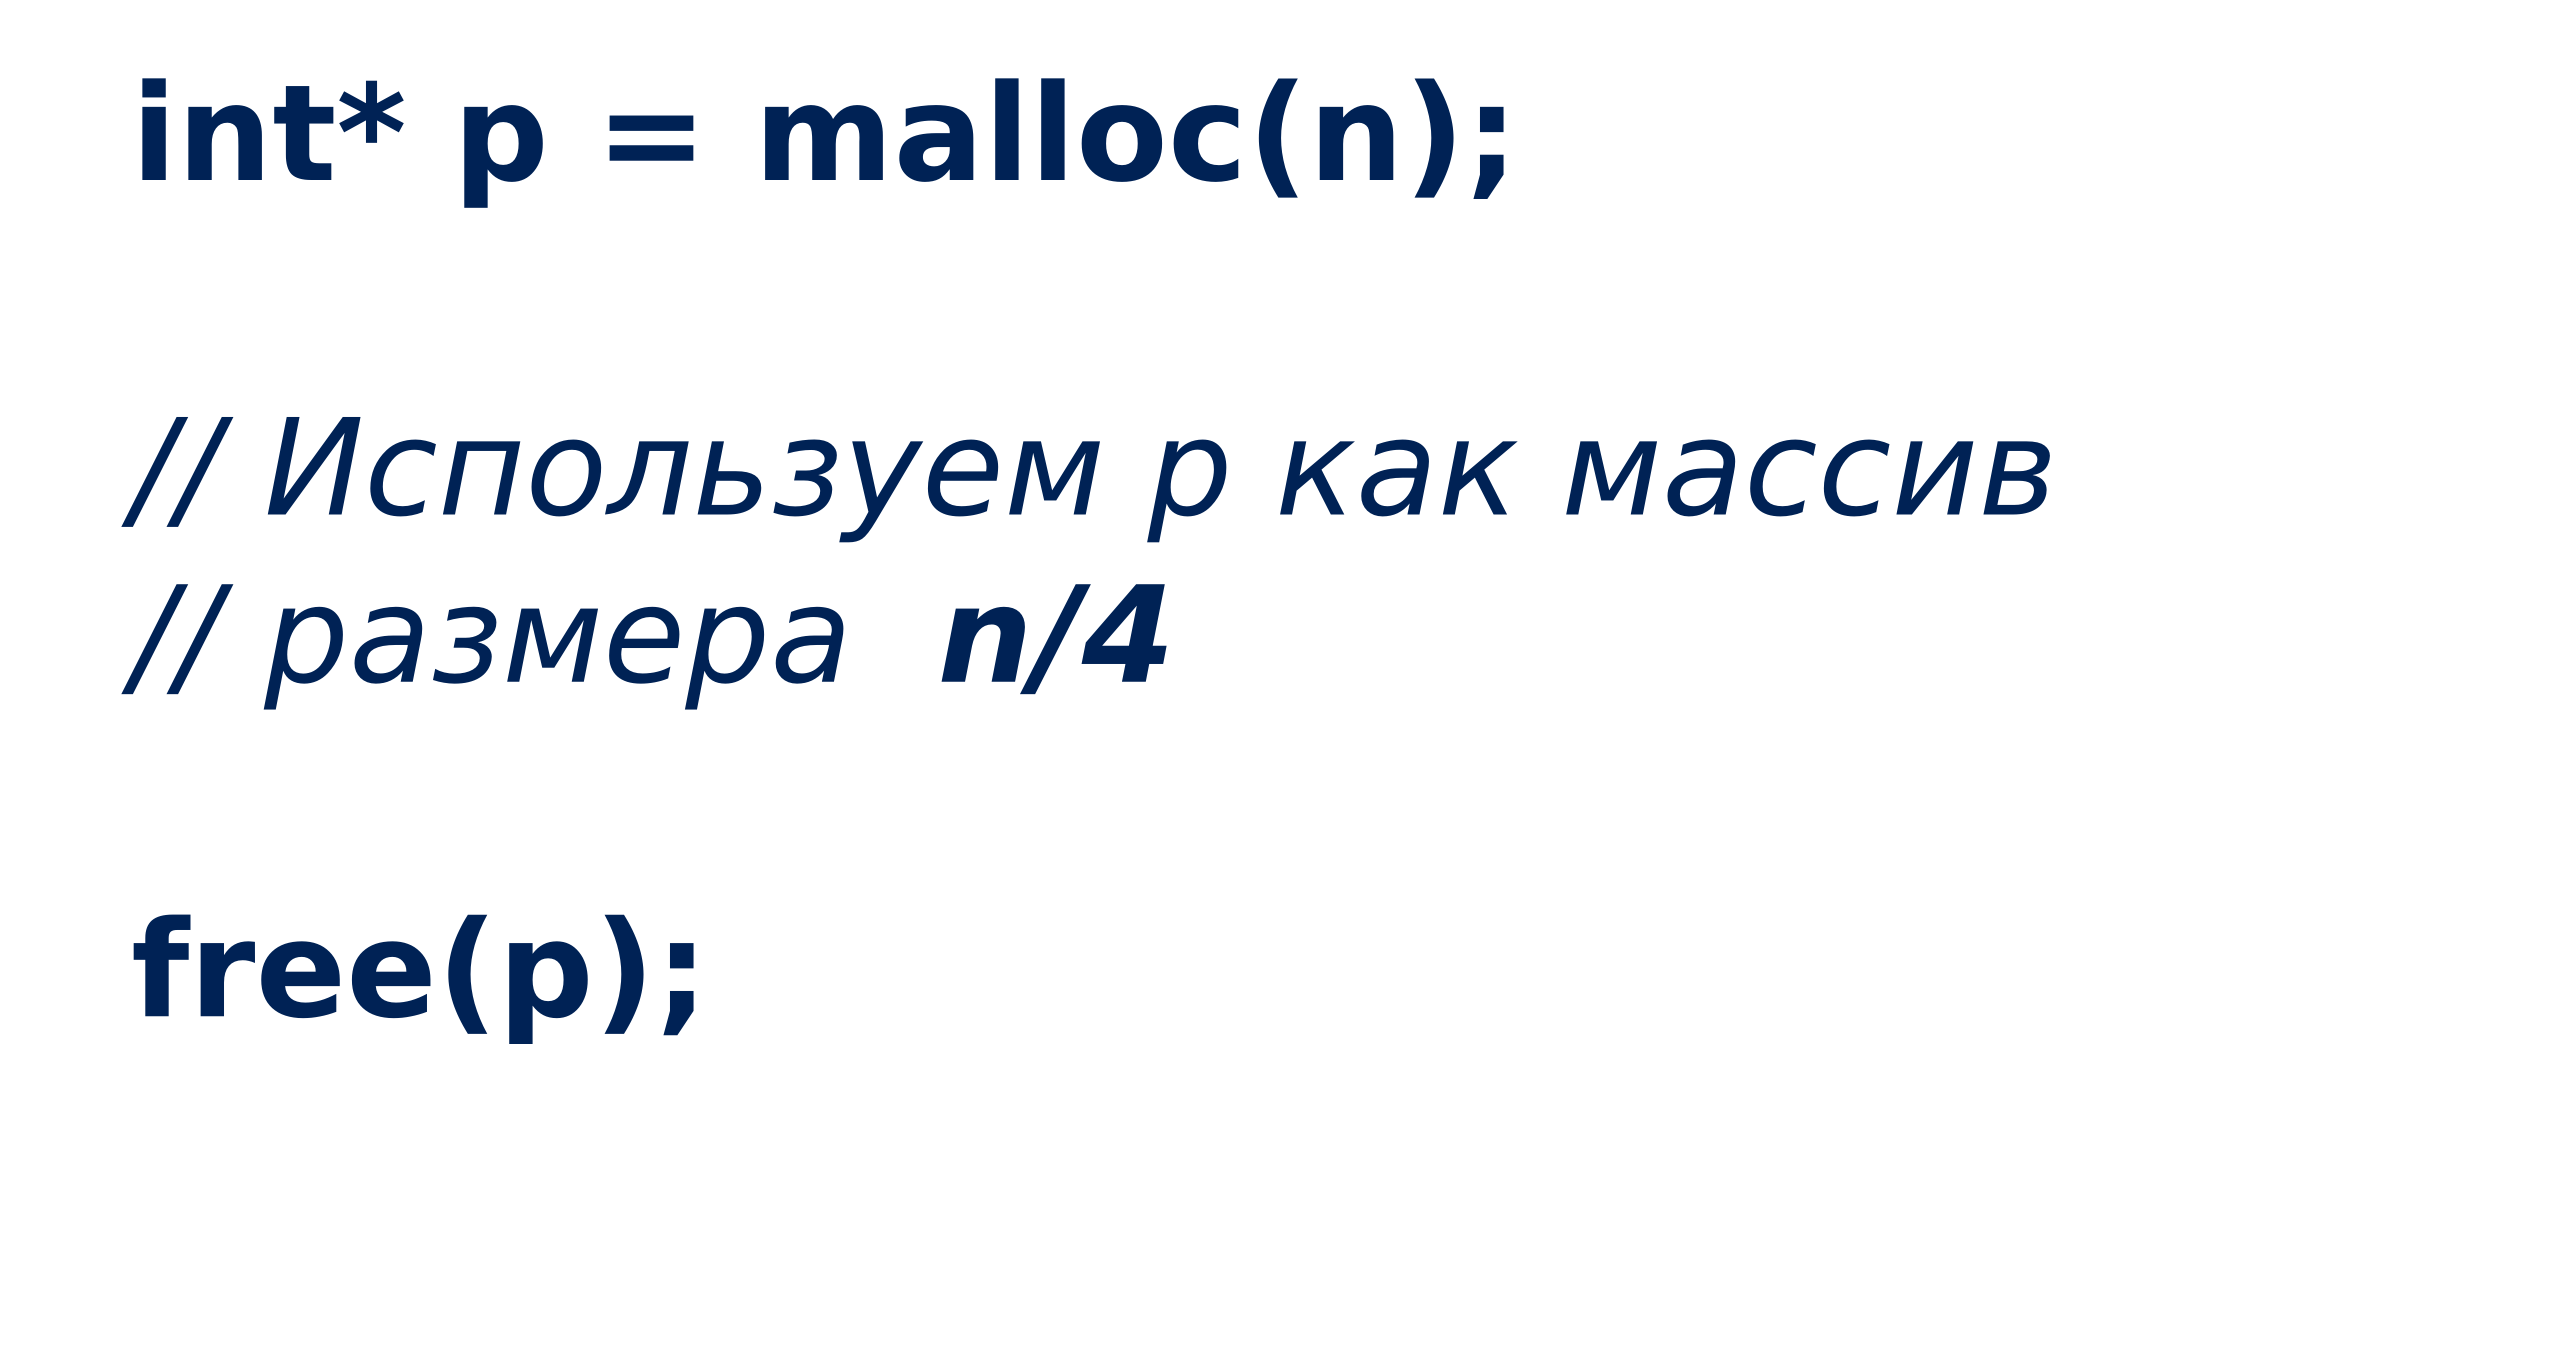
\includegraphics[width=1.0\linewidth]{images/malloc_title_1.png}
\end{center}
\end{frame}

\begin{frame}[fragile]
\frametitle{Malloc} 
\begin{center}
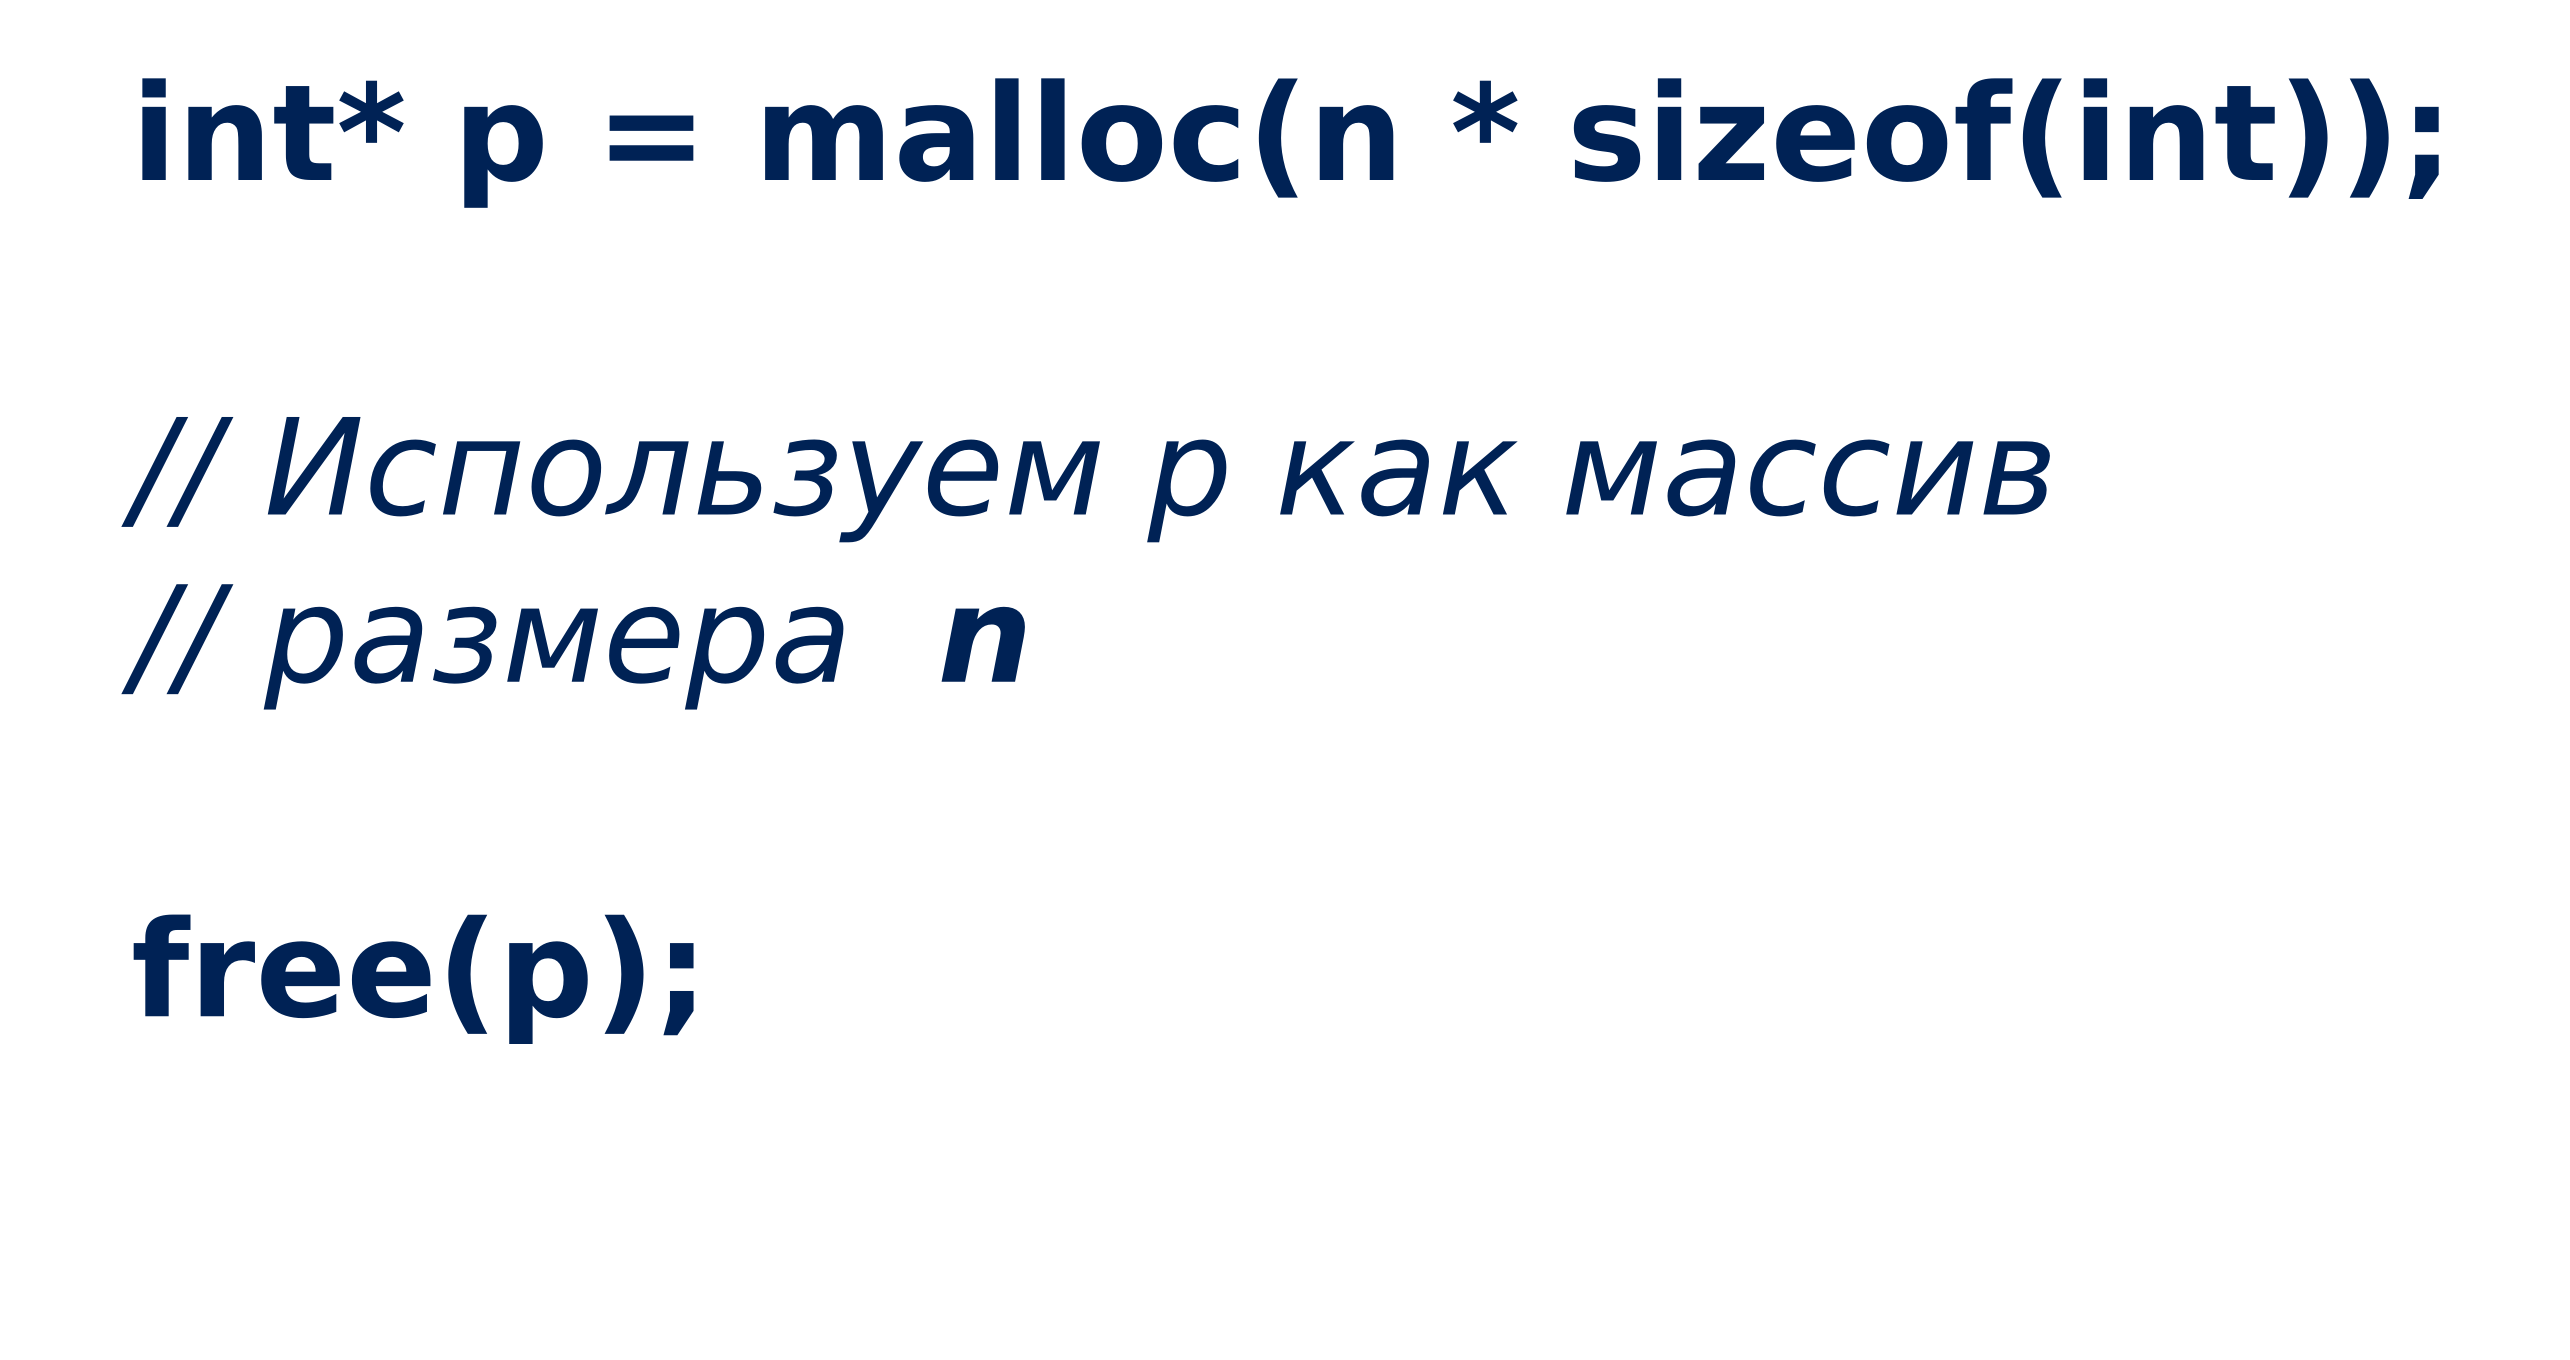
\includegraphics[width=1.0\linewidth]{images/malloc_title_2.png}
\end{center}
\end{frame}

\begin{frame}[fragile]
\frametitle{Malloc} 
\begin{center}
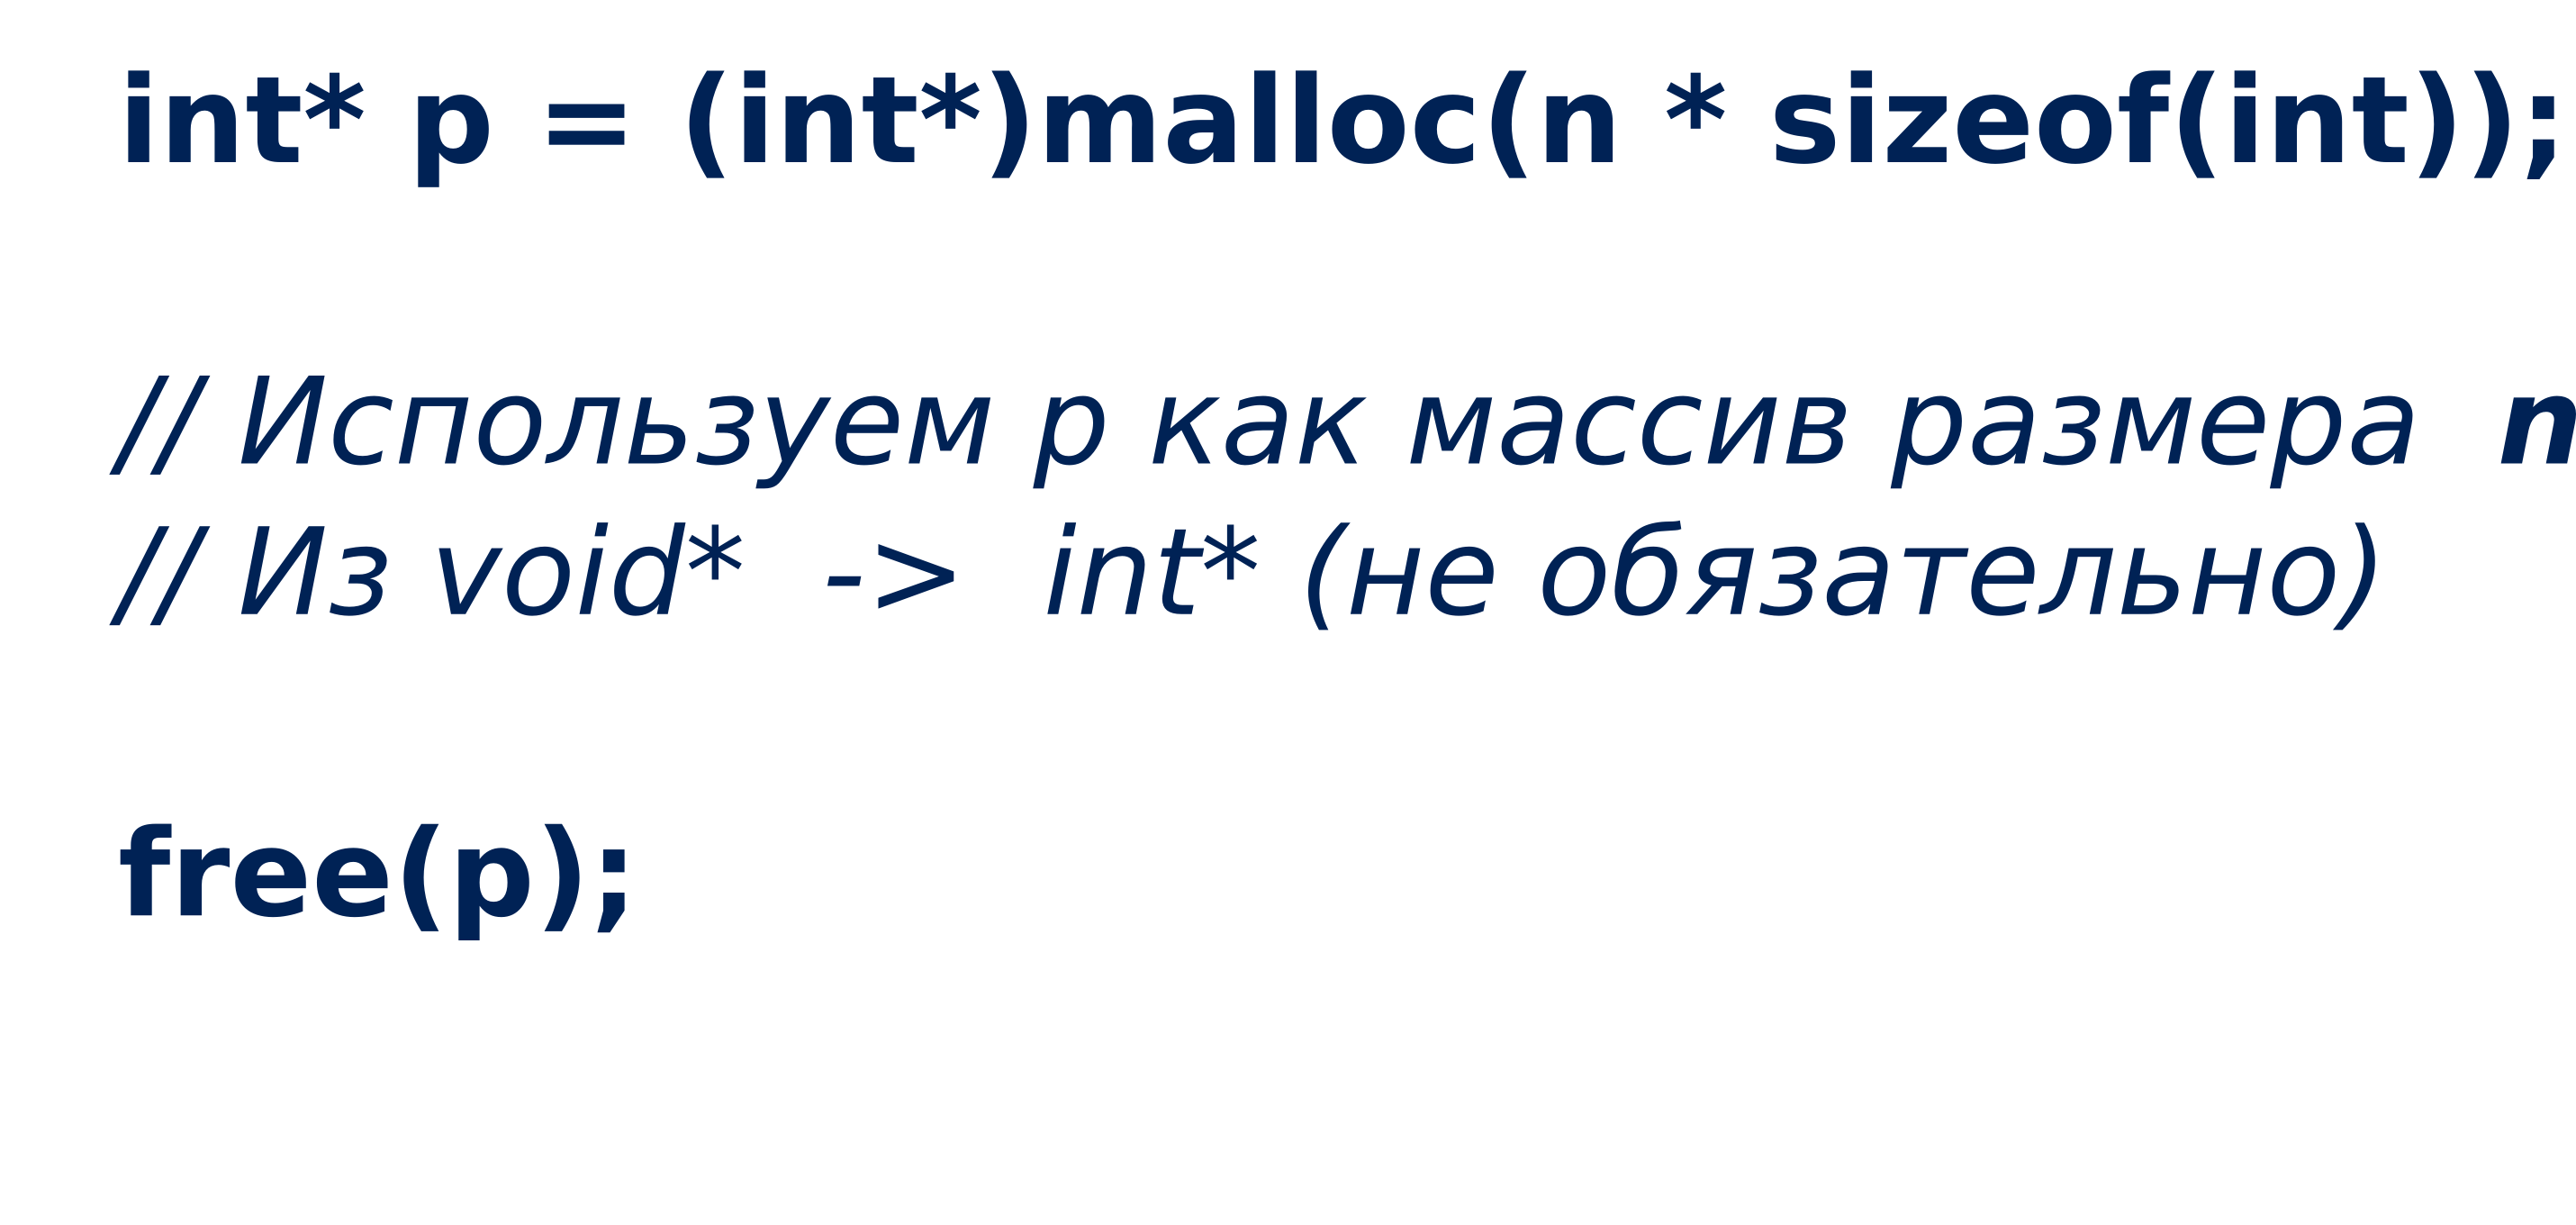
\includegraphics[width=1.0\linewidth]{images/malloc_title_3.png}
\end{center}
\end{frame}




\section{Абстрактные типы данных: стек и очередь}

\begin{frame}[fragile]
\frametitle{Стек} 
\textbf{Стек(stack)} -- абстрактный тип данных, представляющий собой список элементов, организованных по принципу «последним пришёл — первым вышел». 

Операции со стеком:
\begin{itemize}
\item \textbf{push} -- добавляет элемент в вершину стека
\item \textbf{pop} -- удаляет элемент с вершины стека
\end{itemize}
\end{frame}


\begin{frame}[fragile]
\frametitle{Стек} 
\begin{center}
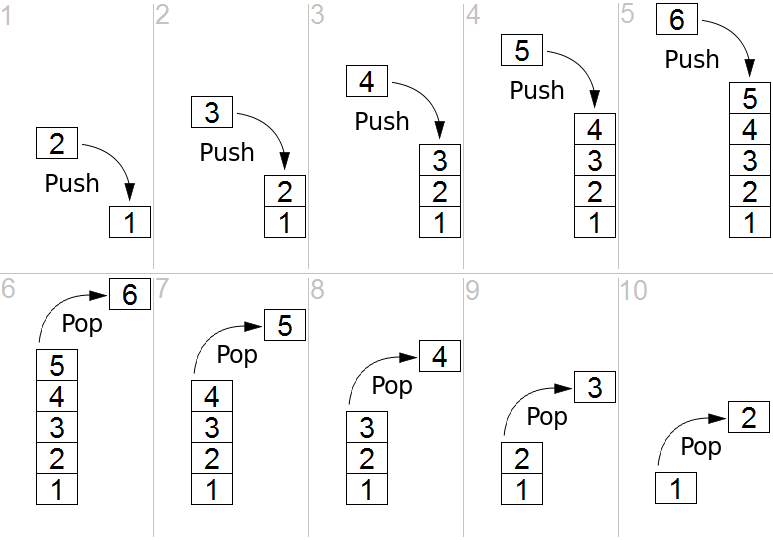
\includegraphics[width=0.8\linewidth]{images/Lifo_stack.png}
\end{center}
\end{frame}


\begin{frame}[fragile]
\frametitle{Стек} 
\framesubtitle{Реализация стека в языке C с помощью массива} 

\begin{lstlisting}[language=C++,basicstyle=\ttfamily,keywordstyle=\color{blue}]
struct stack 
{
    int n;
    int values[100];
};
typedef struct stack Stack;
\end{lstlisting}
\end{frame}


\begin{frame}[fragile]
\frametitle{Стек} 
\framesubtitle{Добавление элемента в стек (без проверки на размер)} 
\begin{lstlisting}[language=C++,basicstyle=\ttfamily,keywordstyle=\color{blue}]
struct stack 
{
    int n;
    int values[100];
};
typedef struct stack Stack;

void stack_push(Stack* s, int x)
{
    s->values[s->n] = x;
    s->n += 1;
}
\end{lstlisting}
\end{frame}

\begin{frame}[fragile]
\frametitle{Стек} 
\framesubtitle{Удаление элемента из стека (без проверки на размер)} 
\begin{lstlisting}[language=C++,basicstyle=\ttfamily,keywordstyle=\color{blue}]
struct stack 
{
    int n;
    int values[100];
};
typedef struct stack Stack;

int stack_pop(Stack* s)
{
    s->n -= 1;
    return s->values[s->n];
}
\end{lstlisting}
\end{frame}

\begin{frame}[fragile]
\frametitle{Стек} 
\framesubtitle{Работа со стеком} 
\begin{lstlisting}[language=C++,basicstyle=\ttfamily,keywordstyle=\color{blue}]
int main()
{
    Stack A;
    stack_create(&A);
    stack_push(&A, 5);
    stack_push(&A, 7);
    stack_push(&A, 3);
    stack_pop(&A);
    printf("%d", stack_pop(&A));
}
\end{lstlisting}
Функция stack\_create() просто устанавливает A.n = 0
\end{frame}

\begin{frame}[fragile]
\frametitle{Очередь} 
\textbf{Очередь (queue)} -- абстрактный тип данных, представляющий собой список элементов, организованных по принципу «первый пришёл — первый вышел». 

Операции с очередью:
\begin{itemize}
\item \textbf{enqueue} -- добавляет элемент в конец очереди
\item \textbf{dequeue} -- удаляет элемент с начала очереди
\end{itemize}
\end{frame}

\begin{frame}[fragile]
\frametitle{Очередь} 
\begin{center}
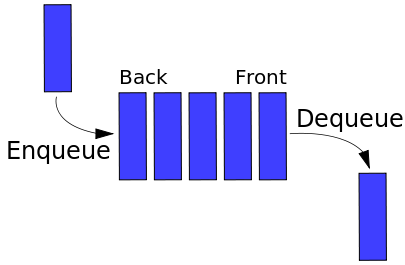
\includegraphics[width=0.8\linewidth]{images/queue_image.png}
\end{center}
\end{frame}


\begin{frame}[fragile]
\frametitle{Очередь} 
\framesubtitle{Реализация очереди в языке C с помощью массива} 
\begin{lstlisting}
struct queue 
{
    int front, back;
    int values[100];
};
typedef struct queue Queue;
\end{lstlisting}
\end{frame}

\begin{frame}[fragile]
\frametitle{Очередь} 
\framesubtitle{Схема реализации очереди с помощью массива} 
\begin{lstlisting}
Queue A;
queue_create(&A);
for (int i = 0; i < 8; ++i)
    enqueue(&A, i*i);
dequeue(&A);
dequeue(&A);
\end{lstlisting}
\vspace{\stretch{200}}    
\begin{center}
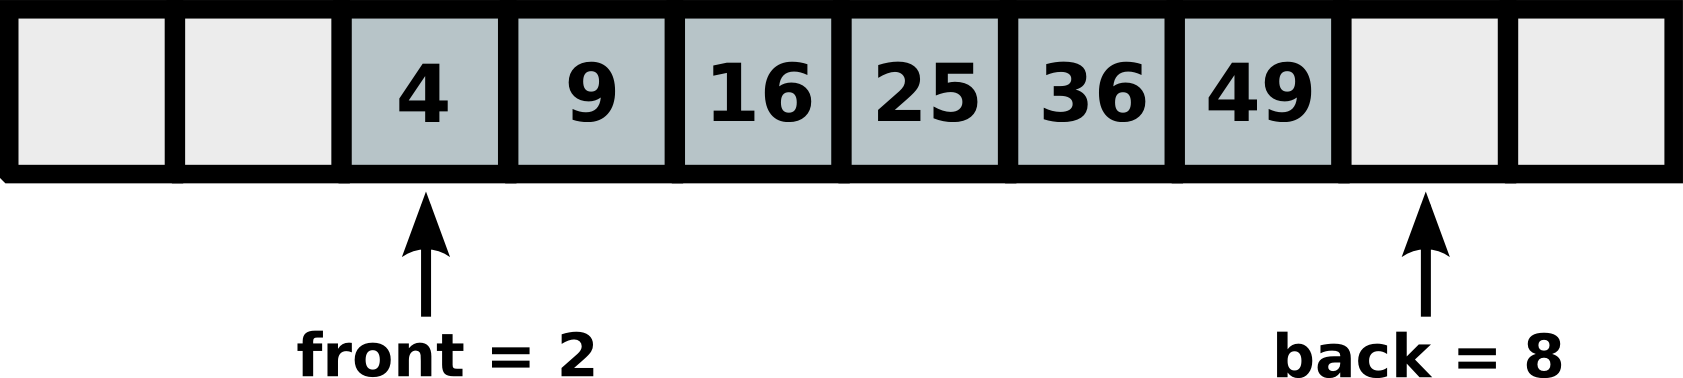
\includegraphics[width=0.8\linewidth]{images/queue1.png}
\end{center}
\end{frame}

\begin{frame}[fragile]
\frametitle{Очередь} 
\framesubtitle{Схема реализации очереди с помощью массива} 
\begin{lstlisting}
dequeue(&A);
dequeue(&A);
\end{lstlisting}
\vspace{\stretch{200}}    
\begin{center}
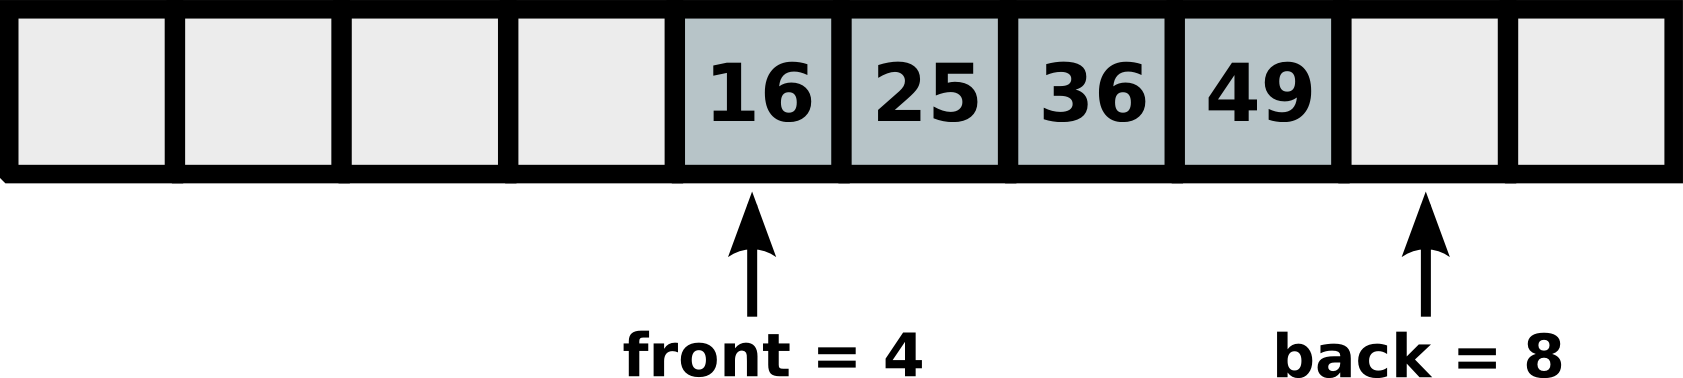
\includegraphics[width=0.8\linewidth]{images/queue2.png}
\end{center}
\end{frame}

\begin{frame}[fragile]
\frametitle{Очередь} 
\framesubtitle{Схема реализации очереди с помощью массива} 
\begin{lstlisting}
enqueue(&A, 9);
enqueue(&A, 2);
enqueue(&A, 5);
\end{lstlisting}
\vspace{\stretch{200}}    
\begin{center}
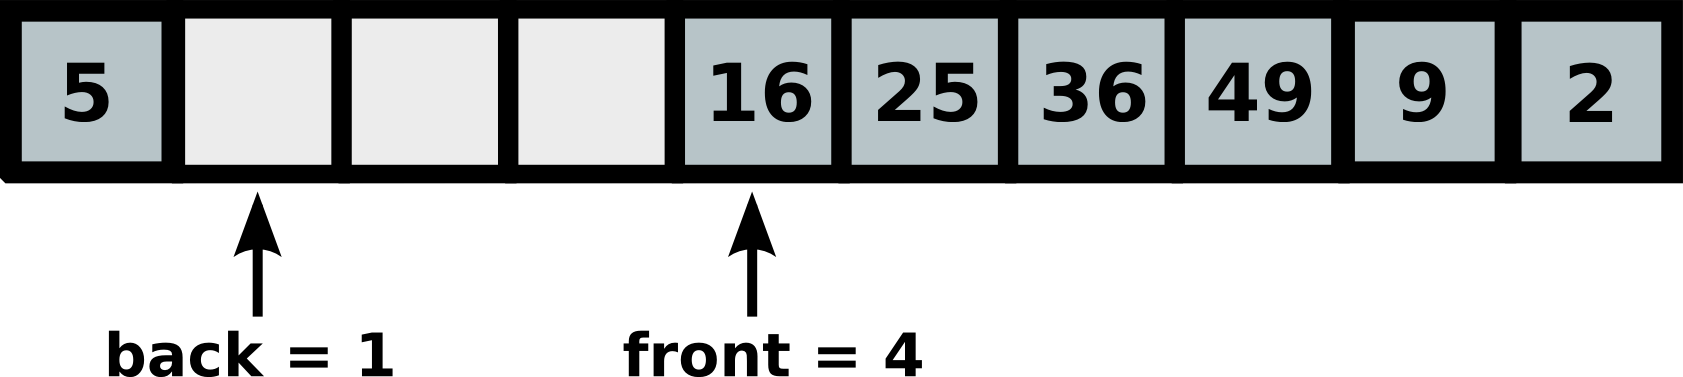
\includegraphics[width=0.8\linewidth]{images/queue3.png}
\end{center}
\end{frame}


\end{document}
